\documentclass[margin=5mm]{standalone}
\usepackage[dvipsnames]{xcolor}
\usepackage{pgfplots}
\usepackage{tikz}
\usepackage[tikz]{ocgx2}

\pgfplotsset{compat=1.18}
\begin{document}

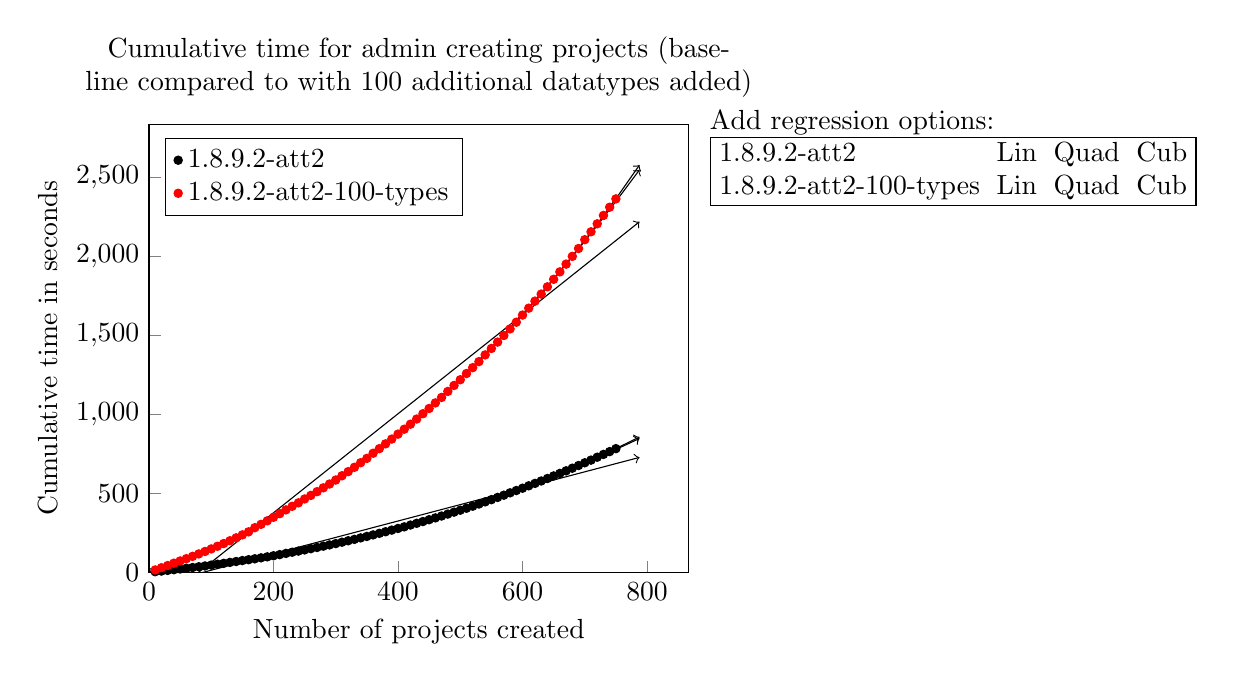
\begin{tikzpicture}
    \begin{axis}[
        align = center,
        legend pos = north west,
        legend cell align = left,
        xlabel = Number of projects created,
        ylabel = Cumulative time in seconds,
        xtick pos = left,
        ytick pos = left,
        scaled ticks = false,
        xmin = 0,
        ymin = 0,
        title = {Cumulative time for admin creating projects (baseline compared to with 100 additional datatypes added)},
        title style = {text width = 0.8\textwidth},
        legend entries={\switchocg{1.8.9.2-att2}{1.8.9.2-att2},\switchocg{1.8.9.2-att2-100-types}{1.8.9.2-att2-100-types}}]
        \begin{scope}[ocg = {ref = 1.8.9.2-att2-Lin, status = invisible}]
            \plot[domain=0:788,->,forget plot] (\x,{-89.42190018017981856246478855609893798828125 + 1.038150719772403363094781525433063507080078125*(\x)^1});
        \end{scope}
        \begin{scope}[ocg = {ref = 1.8.9.2-att2-Quad, status = invisible}]
            \plot[domain=0:788,->,forget plot] (\x,{8.1674016586452413690722096362151205539703369140625 + 0.277714601547792094837774357074522413313388824462890625*(\x)^1 + 0.00100057383976922577295542993169874534942209720611572265625*(\x)^2});
        \end{scope}
        \begin{scope}[ocg = {ref = 1.8.9.2-att2-Cub, status = invisible}]
            \plot[domain=0:788,->,forget plot] (\x,{1.745792235797849922818159029702655971050262451171875 + 0.37587270060901811774556335876695811748504638671875*(\x)^1 + 0.0006798141283382856843442443306457789731211960315704345703125*(\x)^2 + 0.00000028136816792187726049516015465468132816795332473702728748321533203125*(\x)^3});
        \end{scope}
        \begin{scope}[ocg = {ref = 1.8.9.2-att2, status = visible}]
            \addplot[
                only marks,
                color = black,
                mark = *,
                mark size = 1.5 pt
            ]coordinates {(10,4.859)(20,9.023)(30,13.246)(40,17.531)(50,22.13)(60,26.819)(70,31.231)(80,36.331)(90,41.227)(100,46.659)(110,52.301)(120,57.948)(130,63.753)(140,69.436)(150,75.399)(160,80.829)(170,86.599)(180,92.767)(190,98.966)(200,105.993)(210,113.007)(220,120.745)(230,128.206)(240,135.408)(250,142.86)(260,150.738)(270,158.252)(280,166.59)(290,174.483)(300,182.871)(310,191.768)(320,200.827)(330,209.692)(340,218.962)(350,228.177)(360,237.881)(370,247.814)(380,257.892)(390,268.219)(400,278.593)(410,288.864)(420,300.409)(430,311.328)(440,322.592)(450,334.087)(460,345.568)(470,357.451)(480,369.856)(490,382.033)(500,394.329)(510,406.839)(520,419.684)(530,433.481)(540,447.037)(550,460.972)(560,475.33)(570,489.284)(580,504.299)(590,518.816)(600,533.485)(610,548.721)(620,564.024)(630,579.274)(640,595.02)(650,611.236)(660,627.101)(670,643.652)(680,660.174)(690,677.217)(700,694.586)(710,711.448)(720,729.759)(730,747.49)(740,765.275)(750,783.9)};
        \end{scope}
        \begin{scope}[ocg = {ref = 1.8.9.2-att2-100-types-Lin, status = invisible}]
            \plot[domain=0:788,->,forget plot] (\x,{-248.818465225225082804172416217625141143798828125 + 3.134017926031294365429857862181961536407470703125*(\x)^1});
        \end{scope}
        \begin{scope}[ocg = {ref = 1.8.9.2-att2-100-types-Quad, status = invisible}]
            \plot[domain=0:788,->,forget plot] (\x,{19.58136681229149189675808884203433990478515625 + 1.0425906634012938045685814358876086771488189697265625*(\x)^1 + 0.00275187797714473818266878168969924445264041423797607421875*(\x)^2});
        \end{scope}
        \begin{scope}[ocg = {ref = 1.8.9.2-att2-100-types-Cub, status = invisible}]
            \plot[domain=0:788,->,forget plot] (\x,{-1.206065357686601391407066330430097877979278564453125 + 1.3603388619929905889449628375587053596973419189453125*(\x)^1 + 0.00171354470192105318680775294382101492374204099178314208984375*(\x)^2 + 0.000000910818662476916993676044100036737205527970218099653720855712890625*(\x)^3});
        \end{scope}
        \begin{scope}[ocg = {ref = 1.8.9.2-att2-100-types, status = visible}]
            \addplot[
                only marks,
                color = red,
                mark = *,
                mark size = 1.5 pt
            ]coordinates {(10,15.927)(20,30.068)(30,44.002)(40,58.788)(50,72.913)(60,87.438)(70,102.154)(80,117.476)(90,132.968)(100,149.111)(110,166.011)(120,183.21)(130,200.96)(140,219.266)(150,238.23)(160,257.419)(170,283.536)(180,304.819)(190,327.154)(200,349.354)(210,372.305)(220,396.331)(230,419.151)(240,440.869)(250,465.432)(260,487.985)(270,511.593)(280,536.002)(290,559.985)(300,585.273)(310,612.314)(320,638.589)(330,665.988)(340,694.939)(350,722.434)(360,754.886)(370,784.019)(380,814.495)(390,844.727)(400,875.904)(410,907.098)(420,938.835)(430,971.576)(440,1004.988)(450,1038.336)(460,1073.561)(470,1108.173)(480,1146.195)(490,1184.102)(500,1220.273)(510,1259.747)(520,1296.765)(530,1335.01)(540,1377.591)(550,1418.389)(560,1458.697)(570,1500.438)(580,1542.191)(590,1584.5)(600,1629.828)(610,1673.502)(620,1718.041)(630,1762.795)(640,1808.665)(650,1856.283)(660,1903.365)(670,1952.409)(680,2001.538)(690,2051.141)(700,2107.01)(710,2157.063)(720,2207.668)(730,2260.53)(740,2312.548)(750,2365.25)};
        \end{scope}
    \end{axis}
    \begin{scope}
        \addtolength{\tabcolsep}{-0.3em}
        \node [below right, shape=rectangle, align=left](regressiontable) at (7,6) {
            Add regression options: \\
            \begin{tabular}{|llll|}
                \hline
                1.8.9.2-att2 & \switchocg{1.8.9.2-att2-Lin}{Lin} & \switchocg{1.8.9.2-att2-Quad}{Quad} & \switchocg{1.8.9.2-att2-Cub}{Cub} \\
                1.8.9.2-att2-100-types & \switchocg{1.8.9.2-att2-100-types-Lin}{Lin} & \switchocg{1.8.9.2-att2-100-types-Quad}{Quad} & \switchocg{1.8.9.2-att2-100-types-Cub}{Cub} \\
                \hline
            \end{tabular}
        };
    \end{scope}
\end{tikzpicture}

\end{document}